
Para sumarizar as principais vantagens, desvantagens e desempenho do padrão considerado legado pela OGC, a OWS, e a nova família de padrões, OGC API, é necessária a realização de estudos para comparar qualitativamente as duas formas de servir dados geoespaciais e um estudo metodológico quantitativo analisando o desempenho de ambas as implementações.

Para avaliar a escolha de abordagem para desenvolvimento de uma API para uso em SIG serão utilizadas duas categorias de métricas: métricas diretas, que podem ser medidas sem envolver outro atributo ou entidade (consumo de CPU, memória, tempo de execução e tempo de resposta da requisição) e métricas indiretas, obtidas a partir de métricas não mensuráveis (qualidade, complexidade, confiabilidade e manutenibilidade).

A primeira etapa desse trabalho consiste em analisar conceitualmente as principais características desses serviços, realizar um amplo estudo sobre a arquitetura e a evolução de Web Services e  da proposta de API da OGC. Em princípio, a principal diferença entre os dois é a obrigatoriedade do uso de WSDL, SOAP e XML em Web Services, e o fato da OGC API propor o uso de uma API REST e com uso de documentação OpenAPI. Portanto, essa etapa do trabalho também consiste em pesquisar estudos anteriores que comparam essas características utilizando os principais métodos de avaliação de software. A partir disso, a análise requer coletar dados para diferentes variáveis a fim de estudar os progressos da OGC API em viabilizar a implementação de API para disponibilização de dados espaciais.

A segunda etapa consiste na implementação de um Web Service e uma API, para uma mesma aplicação, em conformidade com os padrões definidos pela OGC. Para cada serviço serão utilizadas métricas para comparar as mesmas funcionalidades, com os mesmos dados. A carga de trabalho será obtida utilizando esses protótipos implementados, tanto em um ambiente controlado quanto em uma aplicação real e em produção: com dados geográficos produzidos em centenas de categorias diferentes, resultantes dos subprojetos que compõem o Projeto Brumadinho UFMG e hospedados na IDE da Plataforma Brumadinho UFMG.

% Eu gostaria muito de uma figura, um diagrama que explique as etapas da metodologia. 

\section{Análise Qualitativa}

A conscientização dos desenvolvedores sobre os avanços da OGC API em comparação a OGC Web Services é essencial para a disseminação de seu bom uso, o que garante a interoperabilidade dos dados espaciais, dos quais muitas áreas da pesquisa científica dependem. 
Conduziremos o estudo visando realizar uma análise qualitativa das novas funcionalidades da API OGC e estudar suas limitações, considerando as experiências de outros pesquisadores e desenvolvedores em relação à arquitetura da API OGC. 
Para atingir esse objetivo, uma pesquisa será projetada para buscar respostas às seguintes questões junto à comunidade de desenvolvedores da OGC API:

\begin{itemize}
    \item QP1 - Quais são as vantagens e desvantagens da OGC API e de OGC Web Services?
    \item QP2 - Quanto tempo irá levar para a OGC API se consolidar?
    \item QP3 - Qual é a diferença de funcionalidade que existe entre os padrões?  Qual a lacuna entre os padrões, em termos de funcionalidade?
\end{itemize}

\section{Etapas da Avaliação}

O estudo compreende em coletar a experiência e o perfil de profissionais reais com desenvolvimento de software livre e aberto, assim como a experiência com implementação de API e Web Services em conformidade com a OGC, e coletar a percepção que tiveram dos avanços das padronizações. Assim, a pesquisa foi projetada em três etapas: (1) Coleta de Dados, (2) Planejamento do formulário, e (3) Análise dos Resultados.

% use o tempo futuro aqui

\begin{itemize}
    \item \textbf{Coleta de Dados} - Consiste em coletar artigos publicados que avaliam implementações feitas até então de API, de serviço e cliente de dados, para planejar as perguntas que correspondam a dificuldades experienciadas por desenvolvedores no momento da pesquisa. A partir desses trabalhos foram selecionados sistematicamente 60 desenvolvedores que participaram ativamente na comunidade de desenvolvimento da padronização da OGC API e das primeiras bibliotecas e produtos de software.
    \item \textbf{Planejamento do formulário} - Elaboração de perguntas que viabilizem a coleta do perfil dos desenvolvedores (razões para participar da comunidade de software livre e de código aberto para geoinformática, tempo de experiência na comunidade, numero de usuários do maior projeto que se envolveu, experiência com a OGC API e OGC Web Service). A segunda parte da pesquisa consiste em questões comparando as duas abordagens, de servir dados espaciais, utilizando métricas de engenharia de software selecionados a partir da revisão sistemática de literatura (esforço, desempenho, manutenibilidade e confiabilidade). A terceira parte envolve a percepção sobre o estado presente e o futuro de tecnologias voltadas para servir dados espaciais da Web (abordagens correspondem com as necessidades do mundo moderno, qual a diferença de funcionalidade que existe entre algumas especificações da família OGC API, quanto tempo os desenvolvedores acreditam que irá levar para que a OGC API se consolide). As respostas da pesquisa são anônimas, todas as questões foram opcionais e a maioria delas usavam a Escala Likert com cinco opções de resposta:"Concordo fortemente", "Concordo", "Não concordo ou discordo", "Discordo", "Discordo fortemente". 
    \item \textbf{Análise dos Resultados} - Realizar, a partir das respostas, uma análise dos dados correspondente as questões de pesquisa. Foi conduzido uma análise dos dados para compreender as diferentes percepções baseado na experiência do desenvolvedor.
\end{itemize}

A tabela \ref{tab:survey-questions}, no apêndice, disponibiliza todas as perguntas do formulário.

\section{Análise Quantitativa}

A adoção ampla da OGC API no futuro pressupõe que existam vantagens sobre os Web Services tradicionais tanto do ponto de vista da flexibilidade de uso e incorporação a sistemas, quanto do ponto de vista de desempenho. A comparação de desempenho, no entanto, precisa ser realizada tendo em mente que as implementações da OGC API ainda não são definitivas, em grande parte. Ainda assim, uma análise de seu desempenho poderá demonstrar a necessidade de melhoramentos em alguns aspectos.

Uma metodologia justa para comparar implementações SOAP e REST requer a escolha de uma configuração e dados apropriados para reduzir o viés do benchmark, uma vez que os padrões de Web Service e API não definem como esses serviços devem ser desenvolvidos. Padronizações limitam-se em definir a abordagem e interface, a fim de garantir a interoperabilidade \cite{introows}. Dado esse fato, a escolha de implementação é condicionada na conformidade do software com as normas OGC. Tais implementações devem ser comparadas em ambientes variados para determinar o quanto de influência a implementação e outros fatores de ambiente podem ter sob o tempo de resposta das requisições. A seção seguinte apresenta a metodologia proposta para essa análise.

\subsection{Parâmetros}

Os parâmetros serão escolhidos considerando o contexto desse estudo, no qual avaliamos os fatores que afetam a média de tempo que uma aplicação leva para responder uma requisição GET 
 de uma \textit{Feature Collection}. Além de variar os conjuntos de dados, os parâmetros listados abaixos foram modelados como fator de duas alternativas. Esse fatores foram selecionados considerando as abordagens API e Web Service de SIG.

\begin{itemize}
    \item Abordagem de serviço: Web Service ou API.
    \item Ambiente de execução: ambiente isolado ou ambiente com outras tarefas alocadas.
    \item Armazenamento dos dados: arquivos no sistema de arquivos (p. ex., shapefiles) ou acesso a bancos de dados geográficos (p. ex., tabelas PostGIS).
    \item Tipo e tamanho dos dados: variação de tipos de representação (pontos, linhas, polígonos), com variação no número de vértices, atributos associados, e complexidade geométrica.
\end{itemize}


\subsection{Conjuntos de dados}

A fim de comparar o resultado para diferentes tipos de dados espaciais serão escolhidos diversos conjuntos de dados de naturezas diferentes para atingir os objetivos da comparação. Esse processo de escolha ainda está em desenvolvimento.



% justificar a escolha!
% sao dados de naturezas diferentes, claro, mas me parece que falta um conjunto de (muitos) pontos.  Talvez seja o caso também de ter um conjunto de dados com tipos variados integrados, como um mapa urbano com muitas camadas. Indicar uma pendência nessa decisão para o caso da proposta de dissertação, e não uma certeza com apenas esses dados abaixo.

Até o momento foram escolhidos três conjuntos de dados do mundo real. O primeiro conjunto de dados inclui apenar uma feature que detalha o limite do estado de Minas Gerais, Brasil, um polígono com 130,163 coordenadas. O segundo conjunto de dados contem 35,293 linhas de contorno da região de Brumadinho em Minas Gerais\footnote{Curvas de nível (equidistâncias 20 e 50m), com o número de vértices variando de 10 até 12801 pares de coordenadas, disponível em \url{http://ide.projetobrumadinho.ufmg.br/layers/geonode_data:geonode:curva_nivel_20}}.O terceiro conjunto de dados contem polígonos das edificações da cidade de Belo Horizonte, Minas Gerais, e inclui 740,763 objetos com uma média de 15 vértices por polígono \footnote{Edificação. Disponível em \url{http://geonetwork.pbh.gov.br/geonetwork/srv/por/catalog.search\#/metadata/6ec5d97f-4be2-4889-81f1-4f06c8a66654}}.


\begin{figure}[H]
\centering
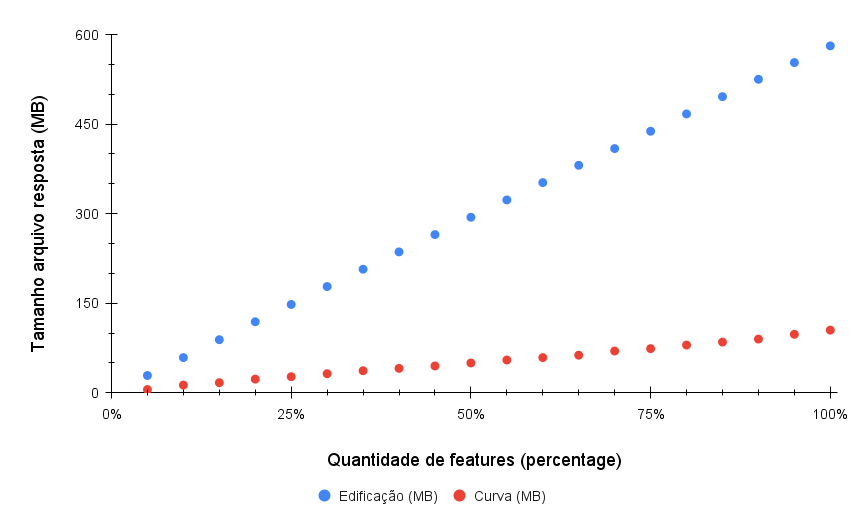
\includegraphics[width=0.8\textwidth]{img/chart.png}
\caption{Crescimento do tamanho do arquivo resposta por porcentagem de features requisitadas para os dois conjuntos de dados escolhidos que possuem mais de uma features}
\label{fig:comparesizes}
\end{figure}


\subsection{Processamento}

A avaliação será realizada sobre os resultados de execução de uma ferramenta de benchmarking HTTP configurada para realizar 50 requisições, sem concorrência, para cada coleção de features. O benchmark será realizado três vezes para cada amostra para garantir a confiabilidade dos tempos de execução obtidos na avaliação.

Para avaliar o efeito do número de features requisitadas e o efeito da abordagem, um Design Fatorial de dois níveis fserá utilizado, o que tornará possível diferenciar como cada fator interfere na performance da abordagem escolhida e estimar o erro exponencial. Para comparar o efeito entre as abordagens e estimar qual performa melhor, um Design Fatorial de um fator é utilizado, já que devemos comparar diversas alternativas de um único fator. A partir dos resultados, uma análise por regressão linear nos permite extrapolar ou interpolar sobre os tempos de resposta de ambas as abordagens e verificar quando uma abordagem prevalece sobre a outra. As técnicas de avaliação utilizadas até então estão disponíveis em \cite{bukh1992art}.
